% !TeX root = main.tex
\documentclass[a4paper,12pt]{scrreport}

\usepackage[ngerman]{babel}

\usepackage[top = 2cm, bottom = 2.5cm, left = 1.5cm, right = 1.5cm]{geometry}

\usepackage{fontspec}
\usepackage{libertine}


\usepackage{fancyhdr}
\pagestyle{fancy}
\fancyhead{}
\fancyhead[LO]{\printauthor}
\fancyhead[RO]{Experiment \arabic{chapter}}

\usepackage{csquotes}

\usepackage{enumitem}

\usepackage{microtype}
\microtypesetup{protrusion=true}
\microtypesetup{expansion=true}

\usepackage{amsmath}


\usepackage{amssymb}
%\numberwithin{equation}{chapter}

\usepackage{siunitx}
\sisetup{locale=DE}

\usepackage{graphicx}

\usepackage{hyperref}
\hypersetup{colorlinks = true, linkcolor = blue}

\usepackage{dsfont}

\usepackage{xcolor}

\usepackage{pdfpages}

\usepackage{float}

\usepackage{booktabs}

\author{\printauthor}
\date{}

\newcommand{\printauthor}{Leonard Scheuer}

\newcommand{\setup}[2]{
	\title{\Huge{ #1: #2} \\ ~ \\ \large{PAP 2}}
	\maketitle
	\tableofcontents
	\setcounter{chapter}{#1}
	%\include{#1.tex}
}

%Abbreviations
\newcommand{\dif}{\text{d}}
\newcommand{\lr}[1]{\left(#1\right)}
\renewcommand{\t}[1]{\text{#1}}

\setcounter{equation}{0}
\author{Leonard Scheuer}
%
\begin{document}
	\setup{221}{Gekoppelte Pendel}

	\section{Motivation/Versuchsziel}
	Wir wollen hier gekoppelte Oszillatoren, in diesem Experiment zwei gekoppelte Pendel, untersuchen. Wir erhalten aus der Theoretischen Betrachtung Lösungen, von welchen wir soche mit bestimmten Anfangsbedingungen näher betrachten (symmetrische, asysmetrische und Schwebungsschwingung) und im Experiment reproduzieren wollen. Die Relevanz dieses Modells geht über den Versuch mit Pendeln weit hinaus, sie ergibt sich aus der breiten Nutzbarkeit von (gekoppelten) Oszillatoren in verschiedenen Bereichen, insbesondere der Festkörperphysik. 
	
	
	\section{Theoretische Grundlagen}
	\subsection{Einzelnes Pendel}
	Zunächst wollen wir kurz ein einzelnes Pendel betrachten, um von diesem bekanntem Gegenstand zum gekoppelten Pendel überzugehen. Bekannt ist für das Drehmoment am Pendel:
	\begin{align}
	M &= I\ddot{\varphi}
\end{align}
wobei $I$ das Trähgeitsmoment des Pendels um die Rotationsachse ist. Nutzen wir, dass für das Drehmemoment auch 
\begin{align}
M= \vec{r} \times \vec{F} = \sin(\varphi)Lmg 
\end{align}
gilt, wobei $L$ die Länge des Pendels ist, so erhalten wir mit Kleinwinkelnäherung:
\begin{align}
	M &=  Lmg \varphi =: -D \varphi
\end{align}
Wobei $D$ als das Direktionsmoment bezeichnet wird. Setzen wir beide Arten gleich, so erhalten wir einen Harmonischen Oszillator, mit bekannter Lösung:
\begin{align}
	&& I\ddot{\varphi} &=  -D\cdot \varphi\\
	 \therefore && \ddot{\varphi} &=  -\frac{D}{I}\cdot \varphi\\
	 \label{eq:om2} \therefore && \varphi(t) &= A \cdot  \cos(\omega\cdot t-\varphi_0),\:\:\omega = \sqrt{\frac{D}{I}} = \sqrt{\frac{g}{L}}
\end{align}
Wobei wir in der letzten Gleichheit das Trägheitsmoment für eine Punktmasse 
\begin{align}
I=mL^2
\end{align}
genutzt haben. 

\subsection{Zwei gekoppelte Pendel}
Koppeln wir nun zwei Pendel mittels einer Feder, wie in Abb. 1 grün, 
so erhalten wir ein Direktionsmoment 

\begin{align}
D' = D_F l^2
\end{align}
wobei $D_F$ die Federkonstante der Feder und $l$ die Entfernung der Aufhängepunkte der Feder zu den Rotationsachsen beschreibt. Daraus resultieren Drehmomente 
\begin{align}
M_1=D'(\varphi_2-\varphi_1)
M_2=D'(\varphi_1-\varphi_2)
\end{align}
Aus der Additivität von Drehmomenten folgt dann ausgehend vom ungekoppelten Pendel:
\begin{align}
	I\cdot \ddot{\varphi_1} = -D\cdot\varphi_1-D'\cdot (\varphi_1-\varphi_2)\notag\\
	I\cdot \ddot{\varphi_2} = -D\cdot\varphi_1-D'\cdot (\varphi_2-\varphi_1)\label{eq:K}
\end{align}
Wir erhalten also zwei gekoppelte Differentialgleichungen. Wir können diese mit den Substitutionen $u=\varphi_1+\varphi_2$ und $v=\varphi_1-\varphi_2$ entkoppeln, sodass :
\begin{align}
	I\ddot{u} &= -Du\\
	I\ddot{v} &= -(D+2D')v
\end{align}
Die Lösungen sind wieder Oszillatorlösungen:

\begin{equation}
\begin{array}{ll}
u=u(t)=A_{1} \cos \omega_{1} t+B_{1} \sin \omega_{1} t & \text { mit }  \omega_{1}=\sqrt{\frac{D}{J}} \\
v=v(t)=A_{2} \cos \omega_{2} t+B_{2} \sin \omega_{2} t & \text { mit }  \omega_{2}=\sqrt{\frac{D+2 D^{\prime}}{J}}
\end{array}
\end{equation}
Durch Rücksubstitution erhalten wir schließlich die allgemeinen Lösungen:
\begin{align}
	\varphi_1(t)&= \frac12\left(A_1\cdot \cos(\omega_1t)+B_1\sin(\omega_1t)+A_2\cdot \cos(\omega_2t)+B_2\sin(\omega_2t)\right) \notag\\
	\varphi_2(t)&= \frac12\left(A_1\cdot \cos(\omega_1t)+B_1\sin(\omega_1t)-A_2\cdot \cos(\omega_2t)-B_2\sin(\omega_2t)\right)\label{eq:phi}
\end{align}
Setzt man bestimmte Anfangsbedingungen ein, so ergeben sich sich die drei hier näher betrachteten Lösungen: 
\subsection{symmetrische Schwingung}
Hier sind Startwinkel beider Pendel identisch und beide ruhen zu beginn. Man sieht leicht, dass \eqref{eq:phi} durch 
\begin{align}
A_1=2\varphi_0 \notag \\ A_2=B_1=B_2=0
\end{align}
gelöst wird. Wir erhalten also 
\begin{align}
	\varphi_{1}(t) &= \varphi_{2}(t) = \varphi_0\cdot \cos(\omega_1t)
\end{align} 
Die Pendel verhalten sich also wie ungekoppelt, was auch aus \eqref{eq:K} direkt ersichtlich ist.
\subsection{asymmetrische Schwingung}
Hier werden die Pendel gegenphasig losgelassen, ruhen aber weiterhin zu Beginn. Analog können wir hier sehen:
\begin{align}
A_2=2\varphi_0 \notag \\ A_1=B_1=B_2=0
\end{align}

\begin{align}
	\varphi_{1}(t) &= - \varphi_{2}(t) = \varphi_0\cdot \cos(\omega_2t)
\end{align} 
Wir sehen also wieder eine harmonische Schwingung, die gegenläufig von beiden Pendeln ausgeführt wird.
\subsection{Schwebungsschwingung}
Hier wird nur eines der Pendel um $\varphi_0$ ausgelenkt. 
Man sieht, dass \eqref{eq:phi} durch 
\begin{align}
A_1=-A_2=\varphi_0 \notag \\ B_1=B_2=0
\end{align}
gelöst wird. Es ergibt sich dann:
\begin{align}
\varphi_1&=\varphi_0\cdot \sin(\frac{\omega_2+\omega_1}2t)\sin(\frac{\omega_2-\omega_1}2t) \\ \varphi_2&=\varphi_0\cdot \cos(\underbrace{\frac{\omega_2+\omega_1}2}_{=:\omega_{I}}t)\cos(\underbrace{\frac{\omega_2-\omega_1}2}_{=:\omega_{II}}t)
\label{eq:Normfr}
\end{align}
Wobei $\omega_{II}$ die Schwebungsfrequenz ist, und $\omega_{I}$ die Frequenz, mit denen die einzelnen Pendel schwingen.
Anschaulich wird in diesem Fall die Energie des zweiten Pendels an das erste abgegeben, bis dieses schließlich schwingt und das zweite ruht. Der Prozess wiederholt sich dann umgekehrt. 
\subsection{Kopplungsgrad}
Wie stark zwei Pendel gekoppelt sind, lässt sich über den \textbf{Kopplungsgrad} ausdrücken: 
\begin{align}
	\kappa &:= \frac{D'}{D'+D}= \frac{T_1^2-T_2^2}{T_1^2 + T_2^2}
\end{align}
wobei $T_i=\frac{2\pi}{\omega_i}$ die Schwingungsdauer der jeweiligen Pendel ist. 

\section{Durchführung}
\subsection{Material}
\begin{itemize}
	\item Zwei Pendel  (Pendelkörper aus Messing, Dichte: $\rho = \SI{7,5}{\g\per\m\cubed}$)
	\item Kopplungsfeder
	\item fest montierter Magnetischer Winkelaufnehmer 
	\item Analog-Digital Wandler
	\item PC (am AD-Wandler)
\end{itemize}
\subsection{Messungen}
\begin{enumerate}
 \item Messaperatur in Betrieb nehmen und Nullabgleich durchführen.
 \item Bestimmung der Eigenfrequenzen der beiden Pendel. Die Pendel werden ungekoppelt leicht angestoßen und einige Zeit schwingen gelassen um die Eigenfrequenz (in der Software) zu bestimmen.
 \item Die drei beschriebenen Anfangspositionen werden jeweils in drei verschiedenen Kopplungsgraden, realisiert durch unterschiedlich hohe Aufhängung der Feder, präperiert und die nachfolgende Schwingung vermessen. 
 \item (optional) Das Verhalten eines Schwingkreises kann qualitativ bei verschiedener Kopplung, realisiert durch Spulenabstände, am Oszilloskop beobachtet werden. (anderer Versuchsaufbau)
\end{enumerate}


\section{Messdaten}
\textit{Siehe nächste Seite}
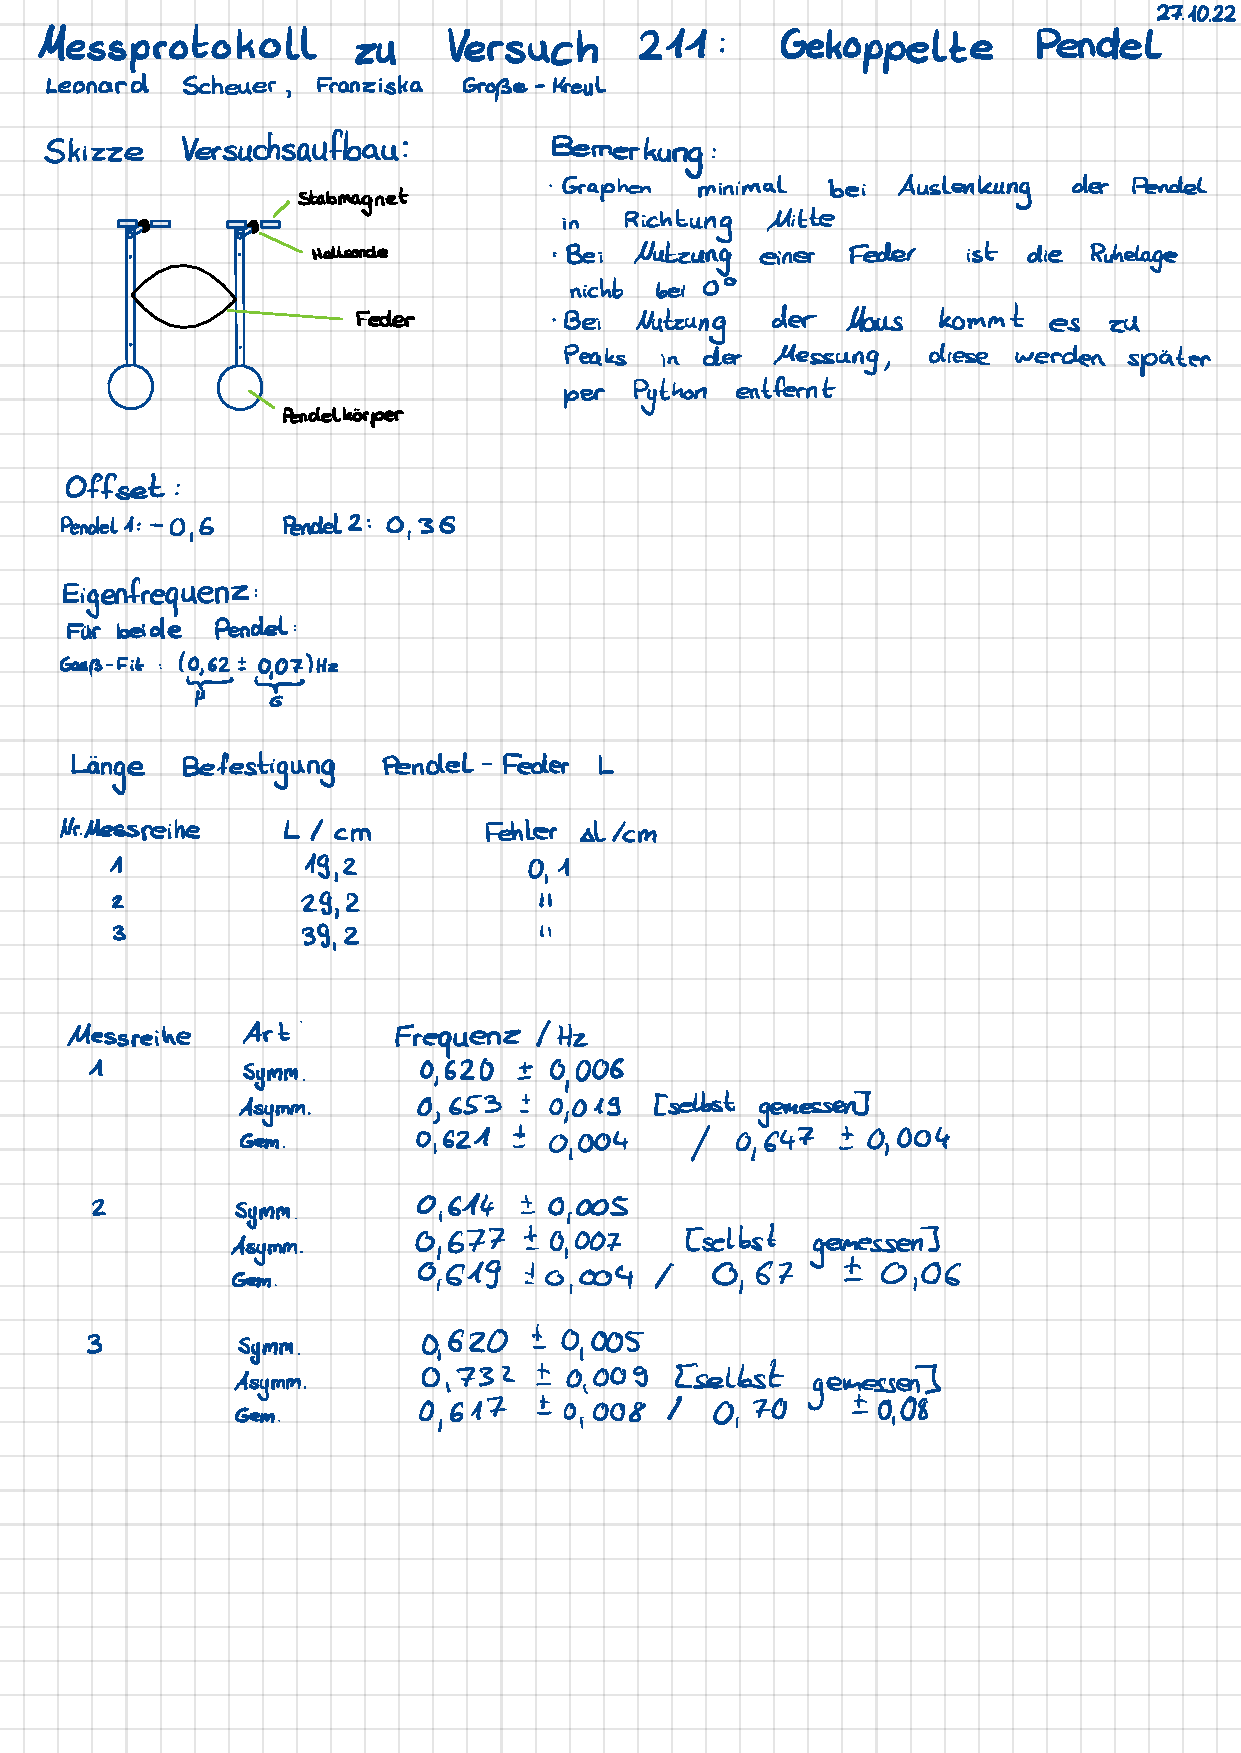
\includepdf[pages=-]{figures/211.pdf}
\subsubsection{Ungekoppelte Schwingung}
\begin{figure}[H]
	\centering
	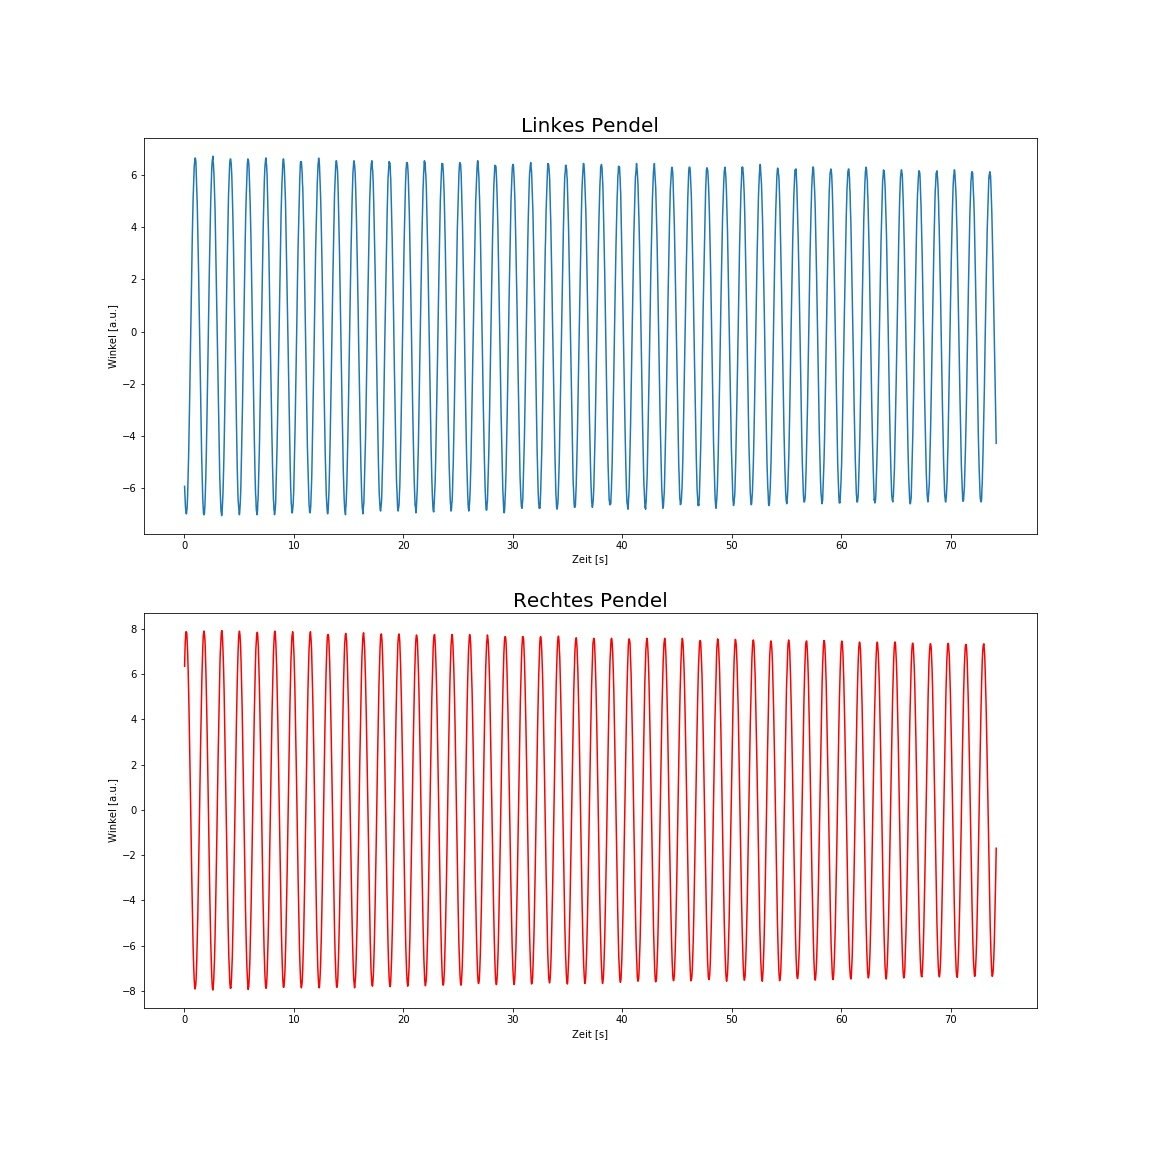
\includegraphics[height = 0.5 \textheight]{figures/211-3.jpeg}
	\caption{Winkelauslenkung in Abhängigkeit von der Zeit, Pendel ungekoppelt}
	%\label{fig:M}
\end{figure}
\begin{figure}[H]
	\centering
	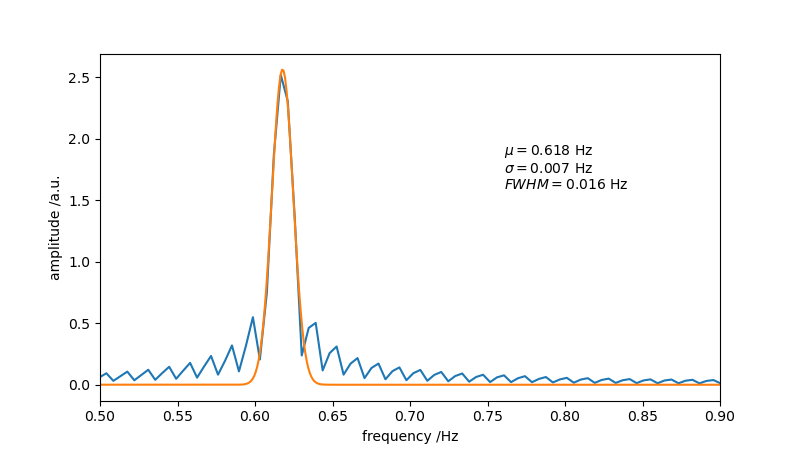
\includegraphics[height = 0.25 \textheight]{figures/211-4.jpeg}
	\caption{Amplitude in Abhängigkeit von der Frequenz, Pendel ungekoppelt}
	%\label{fig:M}
\end{figure}

\subsubsection{Symmetrische Schwingung}
\begin{figure}[H]
	\centering
	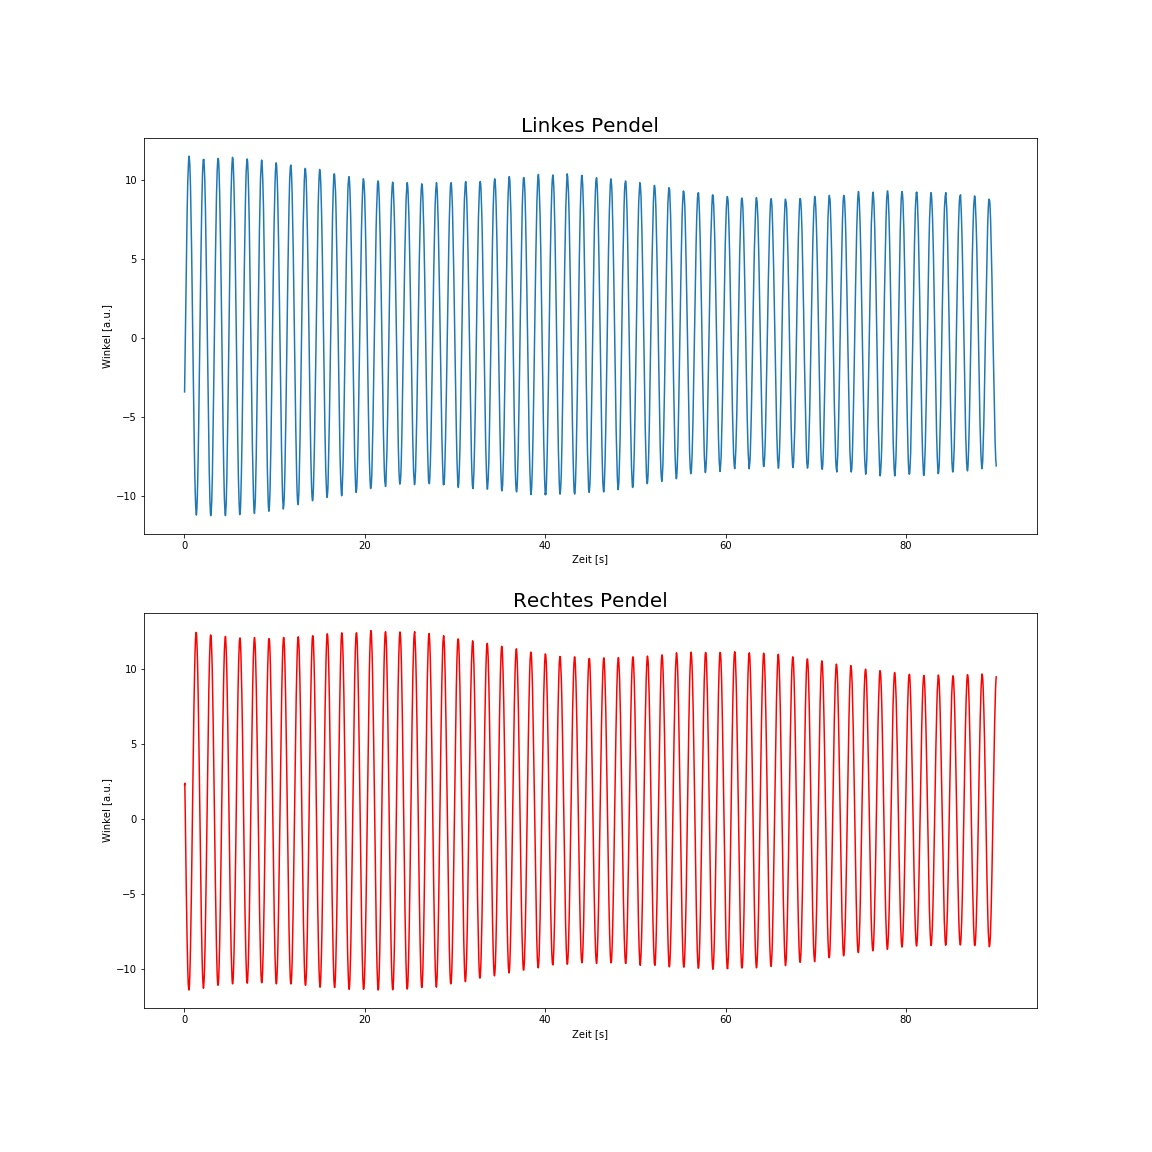
\includegraphics[height = 0.5 \textheight]{figures/211-5.jpeg}
	\caption{Winkelauslenkung in Abhängigkeit von der Zeit, Pendel gekoppelt im Abstand $l = \SI{19,2}{\cm}$ zur Drehachse}
	%\label{fig:M}
\end{figure}
\begin{figure}[H]
	\centering
	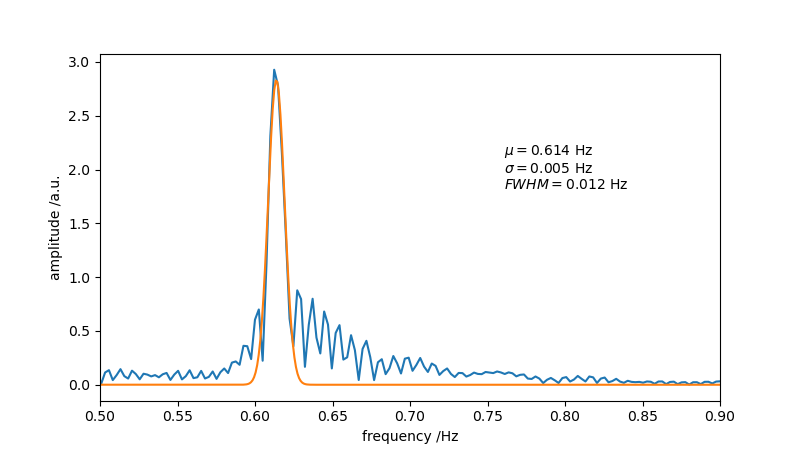
\includegraphics[height = 0.25 \textheight]{figures/211-6.jpeg}
	\caption{Amplitude in Abhängigkeit von der Frequenz, Pendel gekoppelt im Abstand $l = \SI{19,2}{\cm}$ zur Drehachse}
	%\label{fig:M}
\end{figure}

\begin{figure}[H]
	\centering
	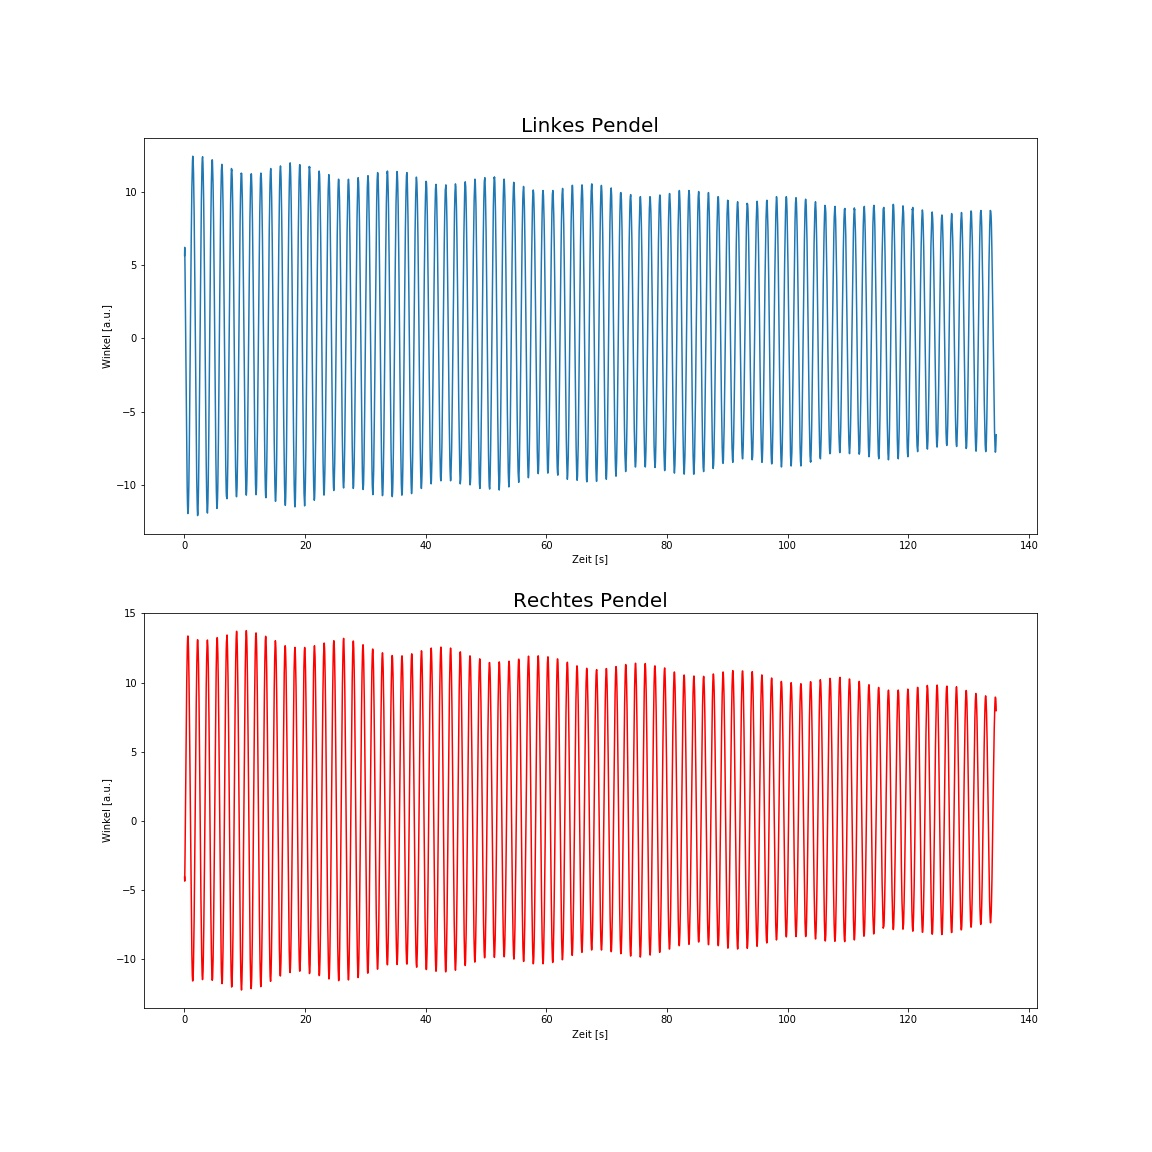
\includegraphics[height = 0.5 \textheight]{figures/211-7.jpeg}
	\caption{Winkelauslenkung in Abhängigkeit von der Zeit, Pendel gekoppelt im Abstand $l = \SI{29,2}{\cm}$ zur Drehachse}
	%\label{fig:M}
\end{figure}
\begin{figure}[H]
	\centering
	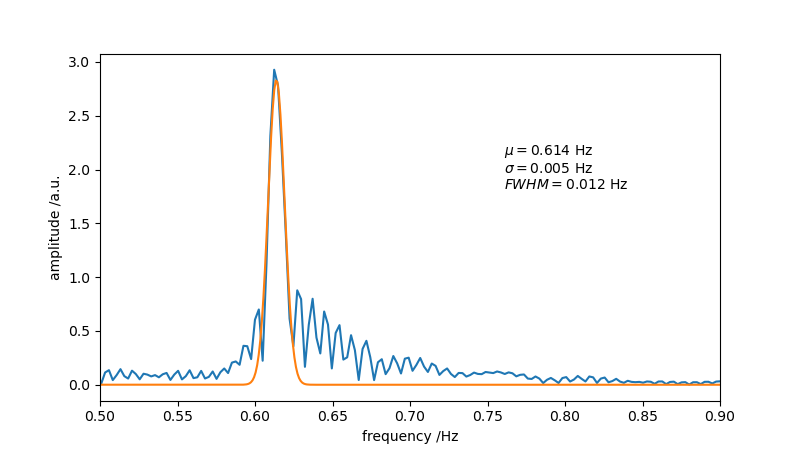
\includegraphics[height = 0.25 \textheight]{figures/211-6.jpeg}
	\caption{Amplitude in Abhängigkeit von der Frequenz, Pendel gekoppelt im Abstand $l = \SI{29,2}{\cm}$ zur Drehachse}
	%\label{fig:M}
\end{figure}

\begin{figure}[H]
	\centering
	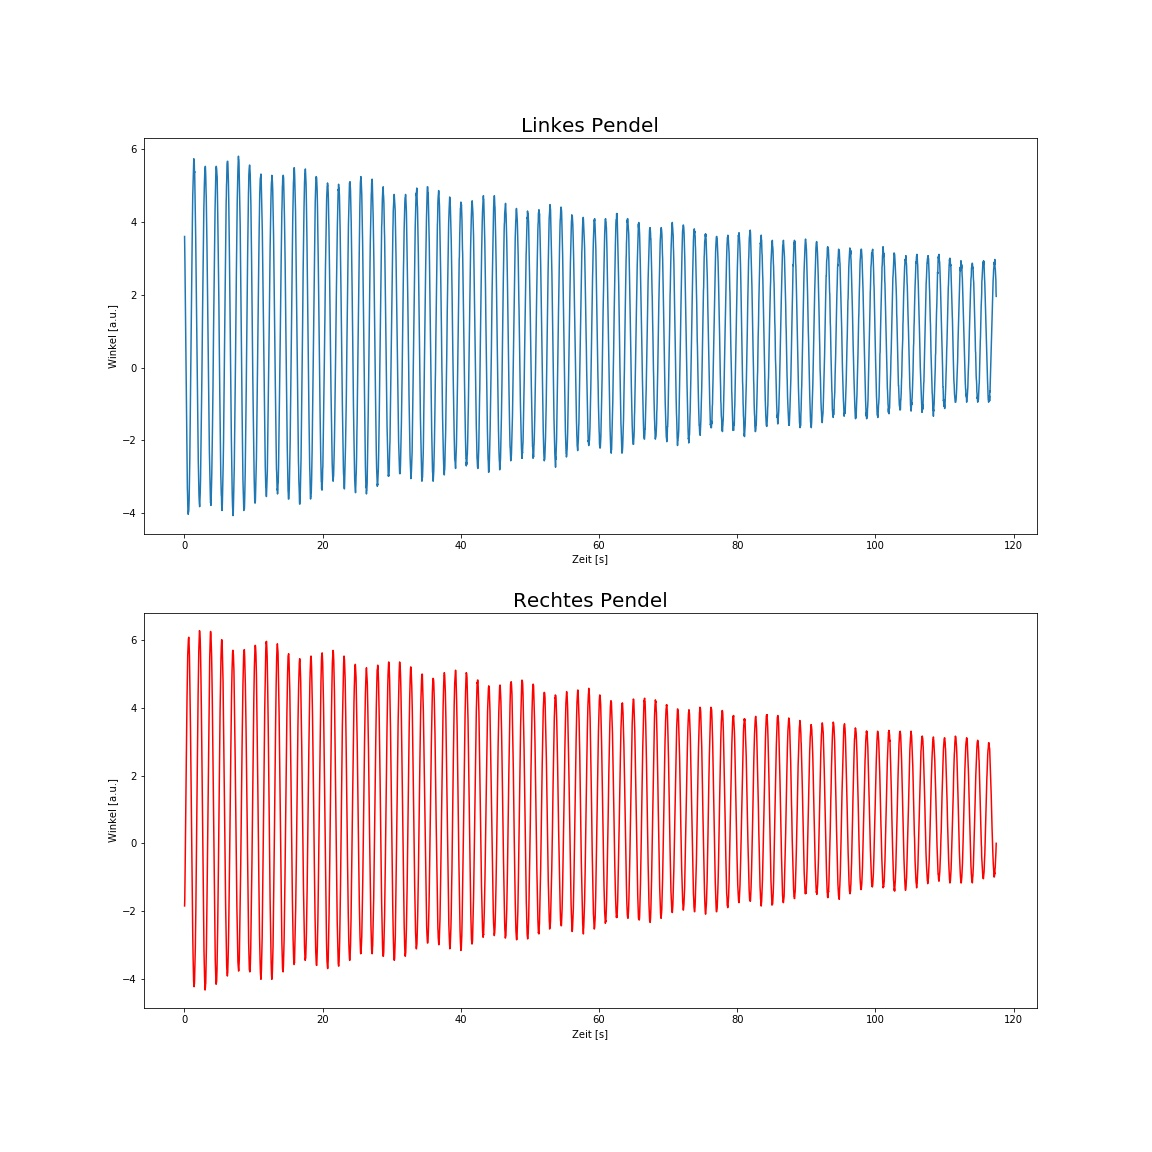
\includegraphics[height = 0.5 \textheight]{figures/211-9.jpeg}
	\caption{Winkelauslenkung in Abhängigkeit von der Zeit, Pendel gekoppelt im Abstand $l = \SI{39,2}{\cm}$ zur Drehachse}
	%\label{fig:M}
\end{figure}
\begin{figure}[H]
	\centering
	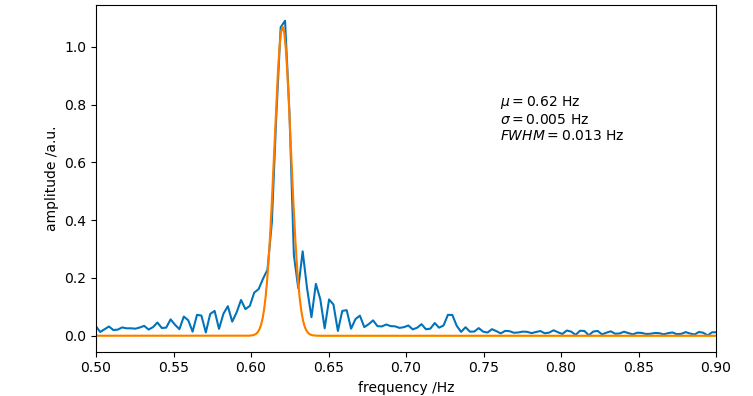
\includegraphics[height = 0.23 \textheight]{figures/211-10.jpeg}
	\caption{Amplitude in Abhängigkeit von der Frequenz, Pendel gekoppelt im Abstand $l = \SI{39,2}{\cm}$ zur Drehachse}
	%\label{fig:M}
\end{figure}


\subsubsection{Asymmetrische Schwingung}
\begin{figure}[H]
	\centering
	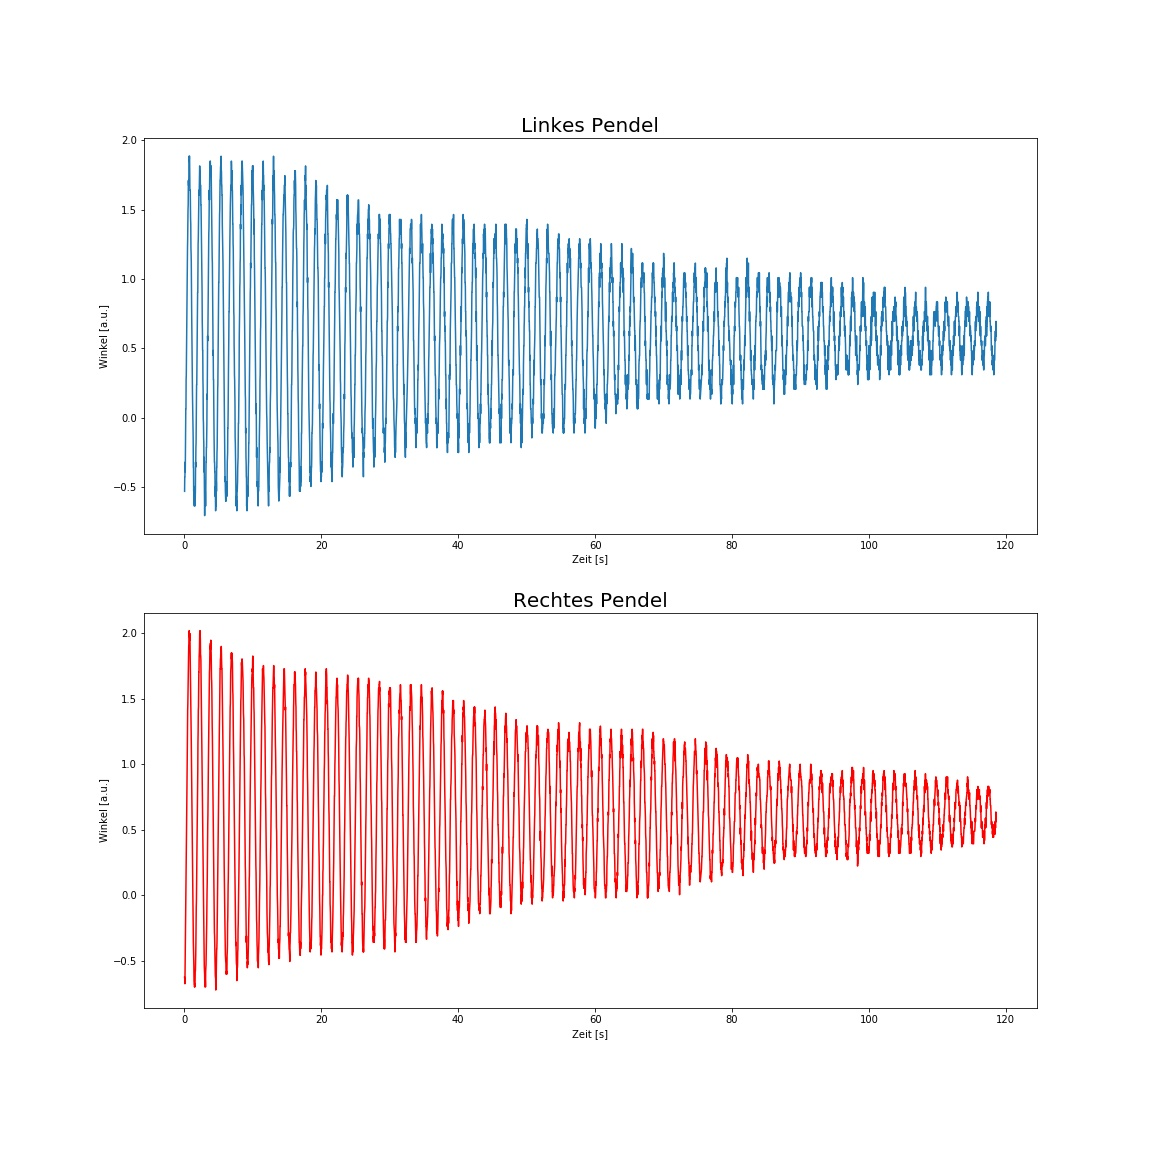
\includegraphics[height = 0.5 \textheight]{figures/211-11.jpeg}
	\caption{Winkelauslenkung in Abhängigkeit von der Zeit, Pendel gekoppelt im Abstand $l = \SI{19,2}{\cm}$ zur Drehachse}
	%\label{fig:M}
\end{figure}
\begin{figure}[H]
	\centering
	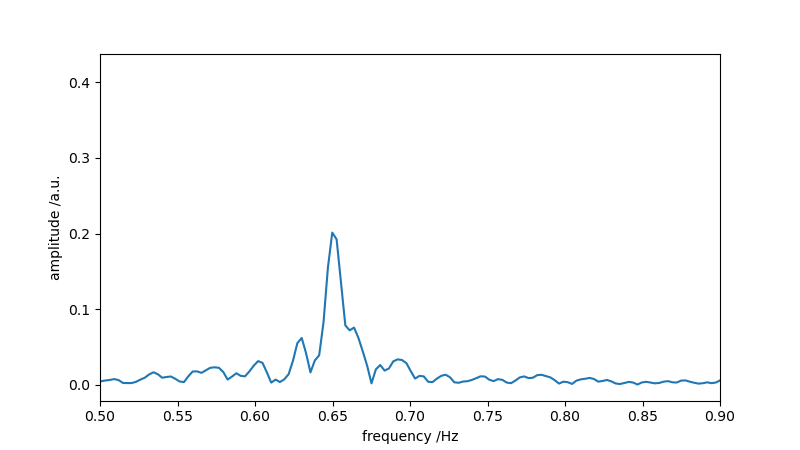
\includegraphics[height = 0.23 \textheight]{figures/211-12.jpeg}
	\caption{Amplitude in Abhängigkeit von der Frequenz, Pendel gekoppelt im Abstand $l = \SI{19,2}{\cm}$ zur Drehachse}
	%\label{fig:M}
\end{figure}

\begin{figure}[H]
	\centering
	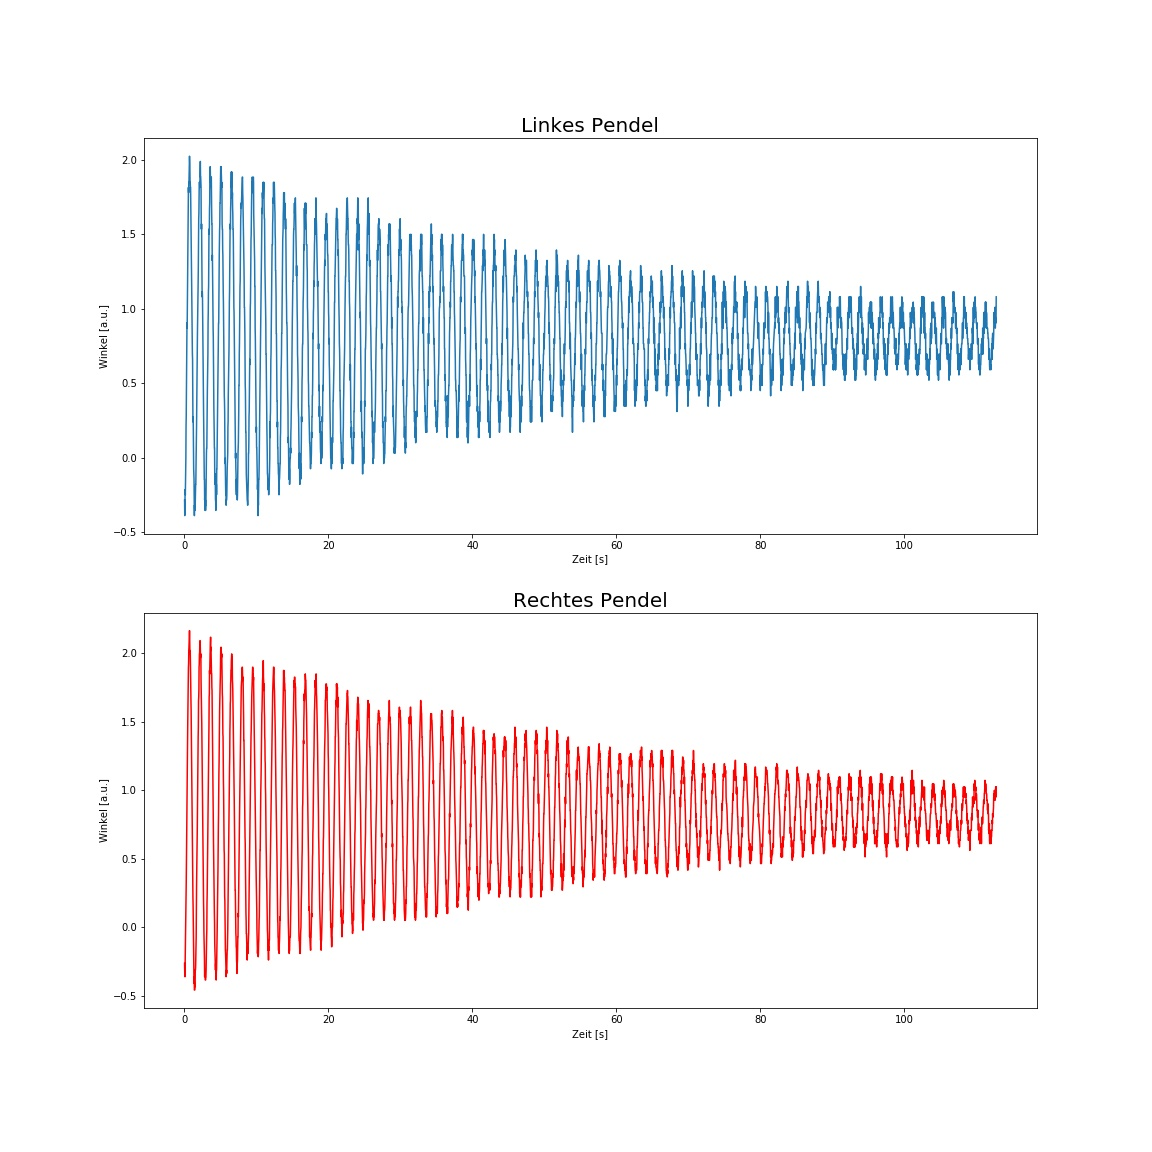
\includegraphics[height = 0.5 \textheight]{figures/211-13.jpeg}
	\caption{Winkelauslenkung in Abhängigkeit von der Zeit, Pendel gekoppelt im Abstand $l = \SI{29,2}{\cm}$ zur Drehachse}
	%\label{fig:M}
\end{figure}
\begin{figure}[H]
	\centering
	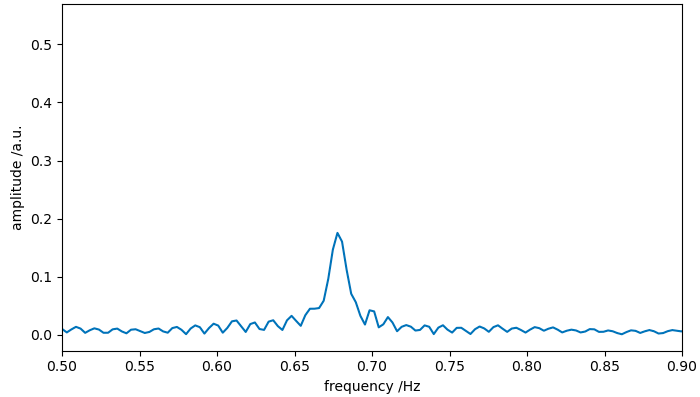
\includegraphics[height = 0.23 \textheight]{figures/211-14.jpeg}
	\caption{Amplitude in Abhängigkeit von der Frequenz, Pendel gekoppelt im Abstand $l = \SI{29,2}{\cm}$ zur Drehachse}
	%\label{fig:M}
\end{figure}

\begin{figure}[H]
	\centering
	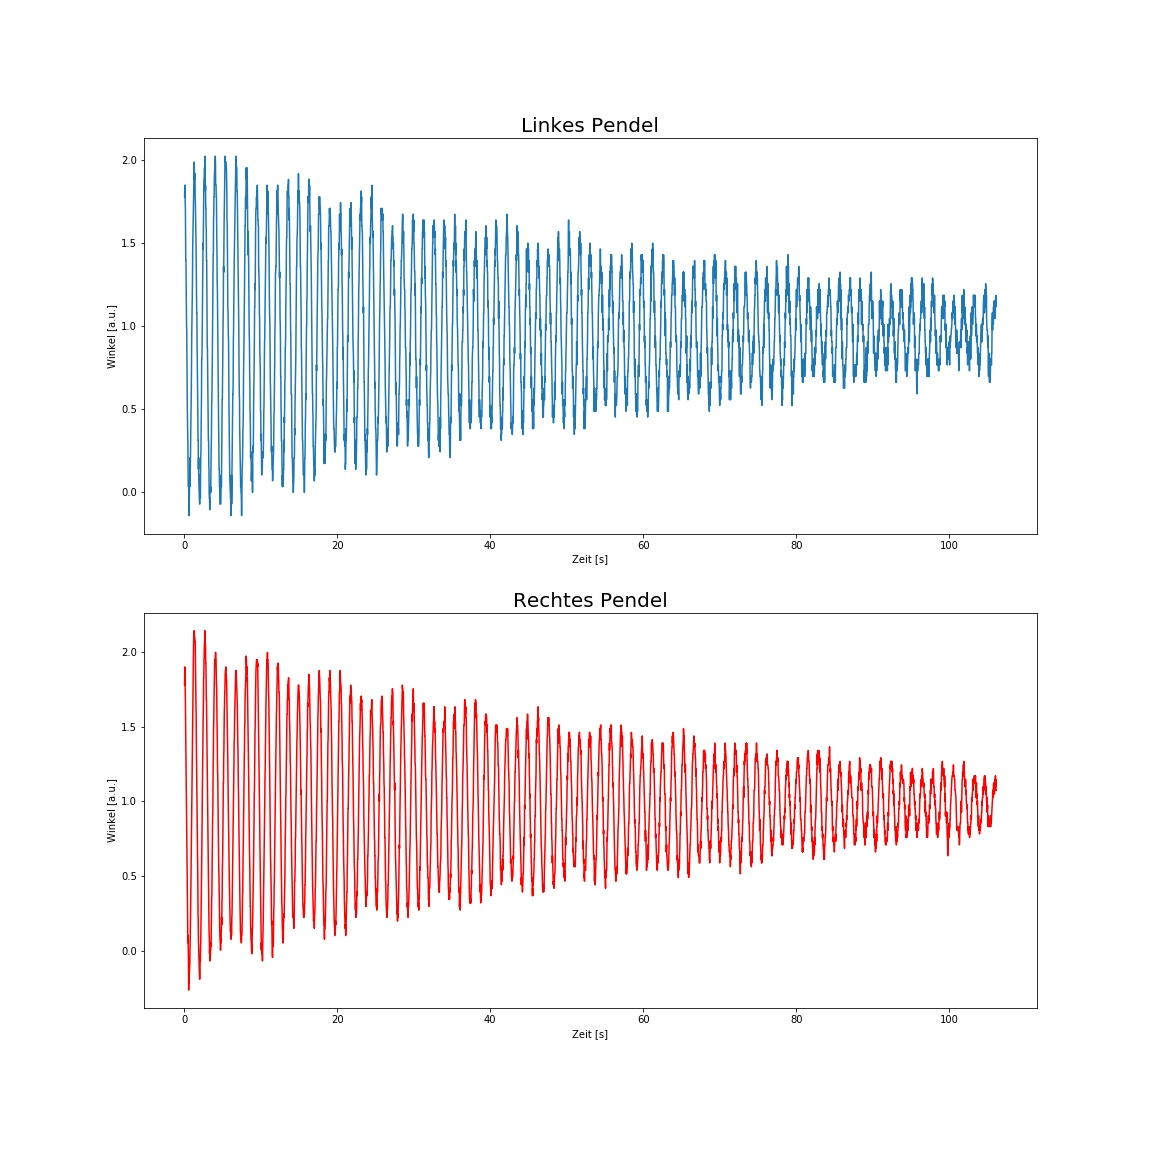
\includegraphics[height = 0.5 \textheight]{figures/211-15.jpeg}
	\caption{Winkelauslenkung in Abhängigkeit von der Zeit, Pendel gekoppelt im Abstand $l = \SI{39,2}{\cm}$ zur Drehachse}
	%\label{fig:M}
\end{figure}
\begin{figure}[H]
	\centering
	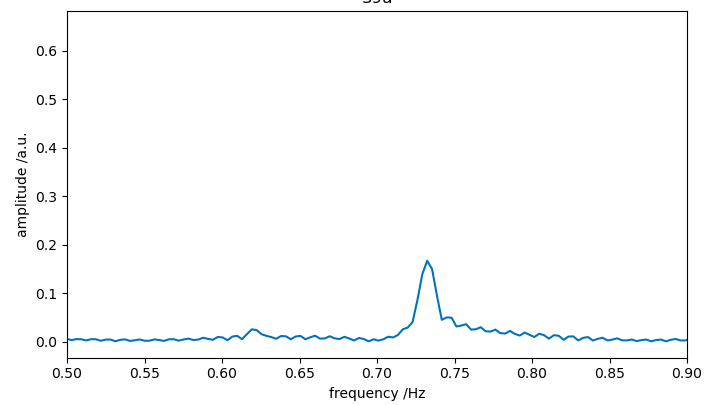
\includegraphics[height = 0.23 \textheight]{figures/211-16.jpeg}
	\caption{Amplitude in Abhängigkeit von der Frequenz, Pendel gekoppelt im Abstand $l = \SI{39,2}{\cm}$ zur Drehachse}
	%\label{fig:M}
\end{figure}


\subsubsection{Schwebungschwingung}
\begin{figure}[H]
	\centering
	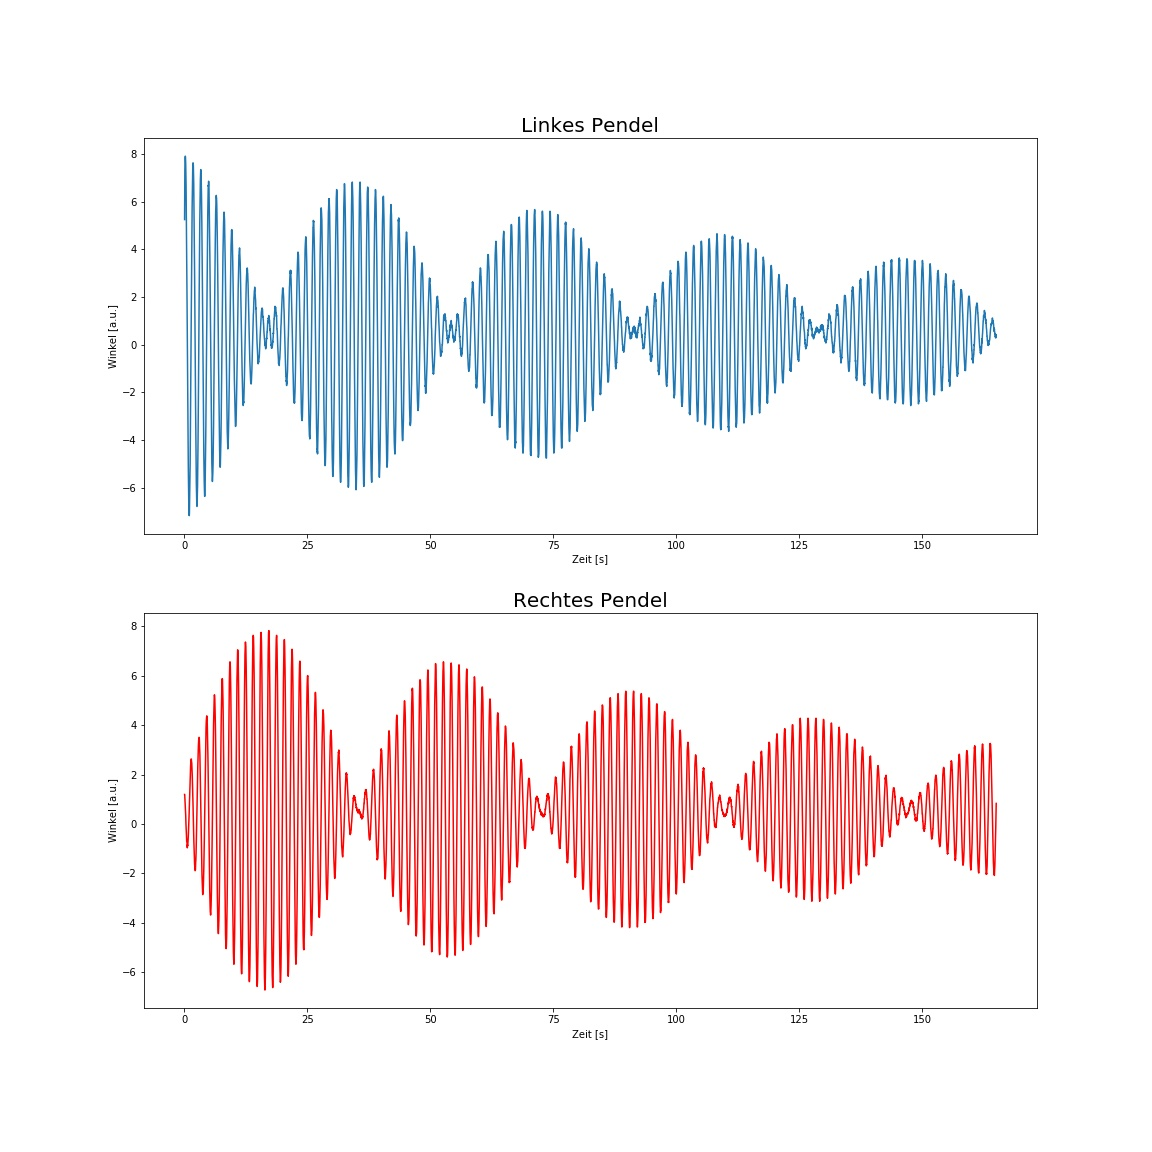
\includegraphics[height = 0.5 \textheight]{figures/211-17.jpeg}
	\caption{Winkelauslenkung in Abhängigkeit von der Zeit, Pendel gekoppelt im Abstand $l = \SI{19,2}{\cm}$ zur Drehachse}
	%\label{fig:M}
\end{figure}
\begin{figure}[H]
	\centering
	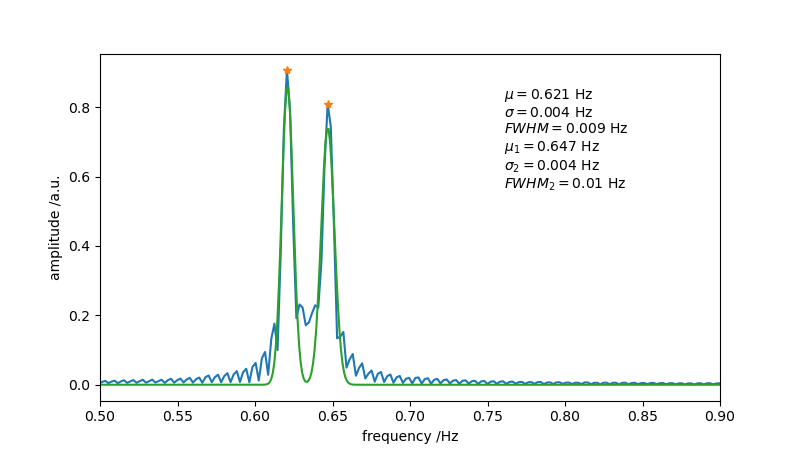
\includegraphics[height = 0.25 \textheight]{figures/211-18.jpeg}
	\caption{Amplitude in Abhängigkeit von der Frequenz, Pendel gekoppelt im Abstand $l = \SI{19,2}{\cm}$ zur Drehachse}
	%\label{fig:M}
\end{figure}

\begin{figure}[H]
	\centering
	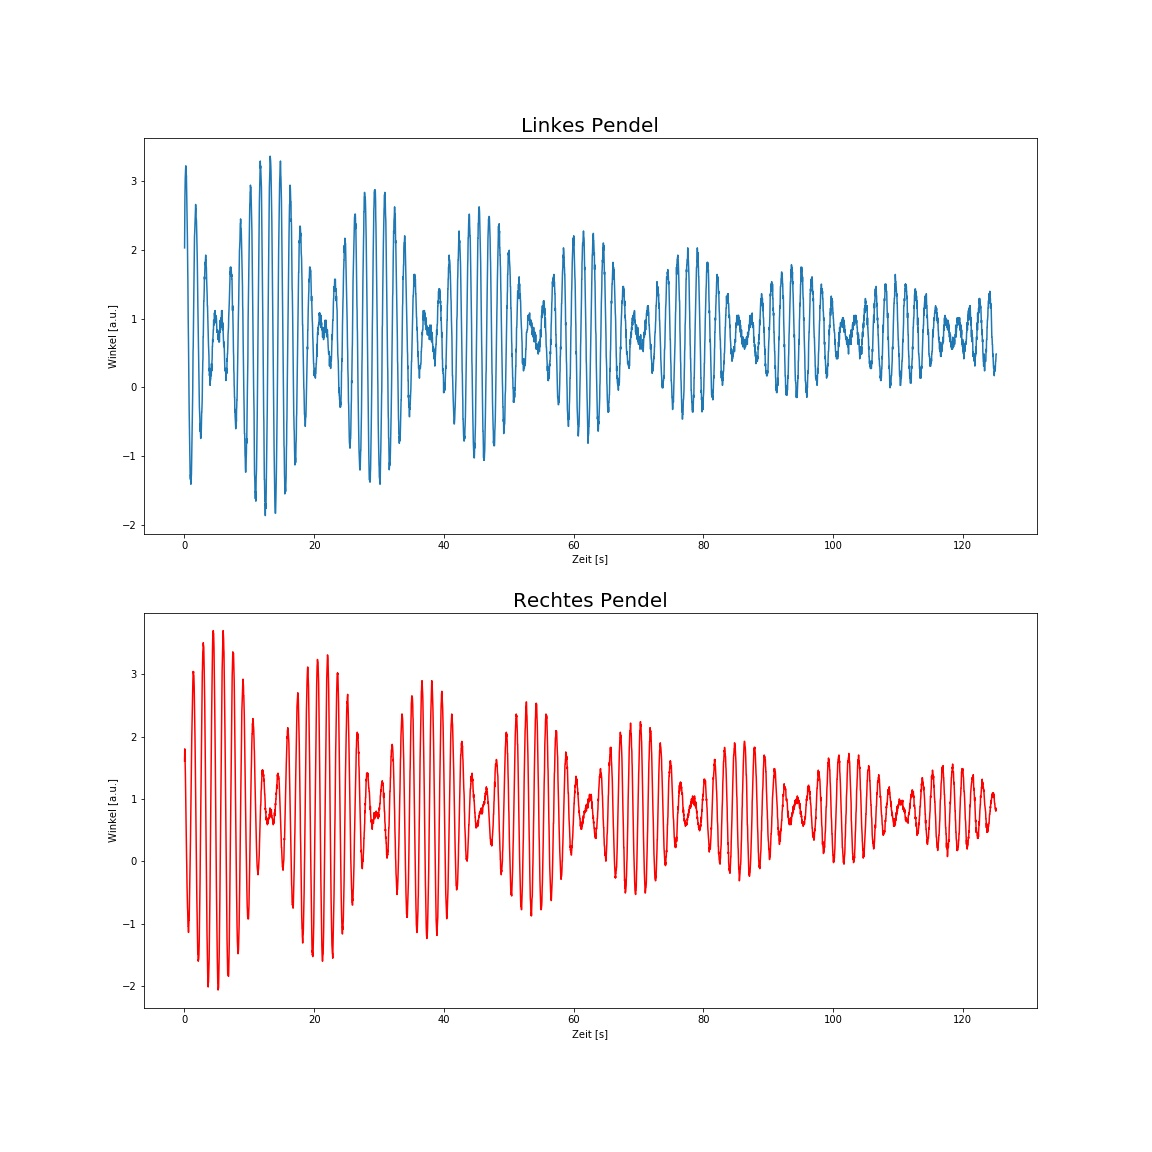
\includegraphics[height = 0.5 \textheight]{figures/211-19.jpeg}
	\caption{Winkelauslenkung in Abhängigkeit von der Zeit, Pendel gekoppelt im Abstand $l = \SI{29,2}{\cm}$ zur Drehachse}
	%\label{fig:M}
\end{figure}
\begin{figure}[H]
	\centering
	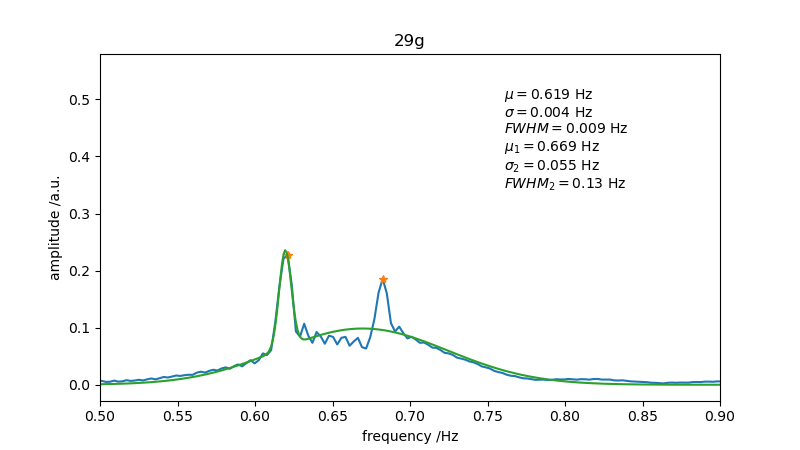
\includegraphics[height = 0.23 \textheight]{figures/211-20.jpeg}
	\caption{Amplitude in Abhängigkeit von der Frequenz, Pendel gekoppelt im Abstand $l = \SI{29,2}{\cm}$ zur Drehachse}
	%\label{fig:M}
\end{figure}

\begin{figure}[H]
	\centering
	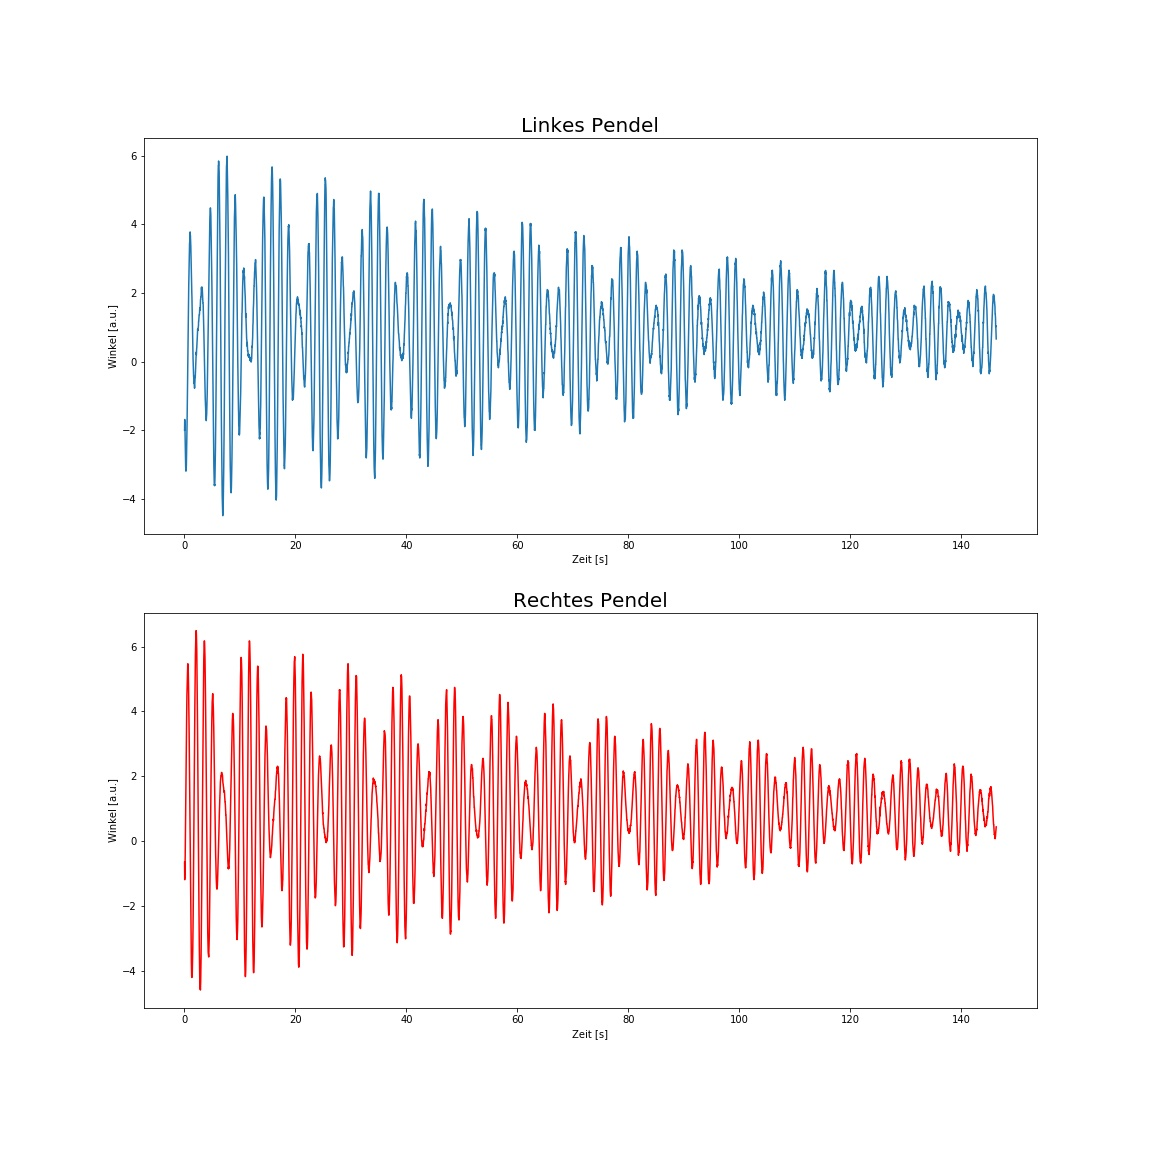
\includegraphics[height = 0.5 \textheight]{figures/211-21.jpeg}
	\caption{Winkelauslenkung in Abhängigkeit von der Zeit, Pendel gekoppelt im Abstand $l = \SI{39,2}{\cm}$ zur Drehachse}
	%\label{fig:M}
\end{figure}
\begin{figure}[H]
	\centering
	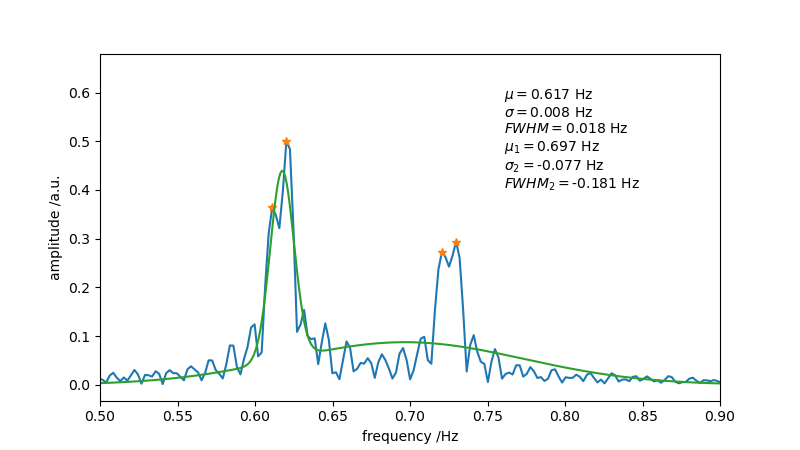
\includegraphics[height = 0.23 \textheight]{figures/211-22.jpeg}
	\caption{Amplitude in Abhängigkeit von der Frequenz, Pendel gekoppelt im Abstand $l = \SI{39,2}{\cm}$ zur Drehachse}
	%\label{fig:M}
\end{figure}



\section{Auswertung}
\subsection{Vergleich der errechneten und gemessenen Frequenzen}
wir nutzen 
\begin{align}
	&& \omega &= 2\pi f\\
	\therefore &&\Delta \omega &= 2\pi \Delta f
\end{align}
Aus \eqref{eq:Normfr} folgt dann sofort:
\begin{align}
	\Delta \omega_{I} &= \Delta \omega_{II}=\frac12 \sqrt{\Delta \omega_1^2+\Delta \omega_2 ^2}
\end{align}
Wir tragen alle Messwerte in eine Tabelle ein und vergleichen $\omega_I$ und $\omega_{II}$ mit den berechneten Werten:
\begin{table}[H]
	\centering
	\begin{tabular}{llllllll}
			$\omega_1$ [Hz] & $\omega_2$ [Hz] & $\omega_I$ [Hz] & $\omega_{II}$ [Hz] & $\frac{\omega_1+\omega_2}{2}$ [Hz] & $\frac{\omega_2-\omega_1}{2}$ [Hz] & $\sigma_{\omega_I}$ & $\sigma_{\omega_{II}}$\\
			\hline
			$3,90 \pm 0,04$ & $4,10 \pm 0,12$ & $3,984 \pm 0,018$ & $0,082 \pm 0,018$  & $4,00\pm 0,06$ & $0,10\pm 0,06$ & 0,26 & 0,29 \\
			$3,86 \pm 0,04$ & $4,25 \pm 0,04$ & $4,05 \pm 0,19$ & $0,16 \pm 0,19$  & $4,055\pm 0,023$ & $0,195\pm 0,023$ & 0,026 & 0,18 \\
			$3,90 \pm 0,03$ & $4,59 \pm 0,06$ & $4,13 \pm 0,25$ & $0,26 \pm 0,25$  & $4,24\pm 0,03$ & $0,35\pm 0,03$ & 0,4 & 0,4 \\
	\end{tabular}
	\caption{Gemessene Kreisfrequenzen und Vergleich mit errechneten Schwebungsfrequenzen}
	\label{tab:1}
\end{table}









\end{document}
